% chapter 2
% Last edit: 2017-5-4
% Modified in Version 1.02 -- 2018-1-18
\chapter{Probability}
\section{Sample Spaces and Events}

\begin{defn}
  An \textbf{experiment} is any action or process that generates observation.
\end{defn}

\begin{exmp}
  Flip a coin once, observe either H or T.
\end{exmp}

\begin{exmp}
  Roll a dice, observe one one spot, two spot \dots six spot.
\end{exmp}

\begin{exmp}
  Choose a card from a well-shuttled deck, observe a deck of cards.\footnote{Four suits: $\spadesuit$spade; $\heartsuit$heart; $\diamondsuit$diamond; $\clubsuit$club. 13 cards in each suit: A,2,3,\dots,10,J,\\Q,K.}
\end{exmp}

\subsection{The Sample Space of an Experiment}
\begin{defn}
  \textbf{Sample space} of an experiment, denoted by $\mathcal{S}$, is the set of all possible outcomes of the experiment.
\end{defn}

\begin{exmp}
  $\mathcal{S}=\{\text{H},\text{T}\}$
\end{exmp}

\begin{exmp}
  $\mathcal{S}=\{1,2,3,4,5,6\}$
\end{exmp}

\begin{exmp}
  $\mathcal{S}=\{A\spadesuit,2\spadesuit ,\dots, K\heartsuit\}$
\end{exmp}

\begin{exmp}
  Flip a coin twice, $\mathcal{S}=\{\text{HH},\text{HT},\text{TH},\text{HH}\}$
\end{exmp}

\subsection{Events}
\begin{defn}
  An \textbf{event} is a collection of outcomes of the sample space, denoted by $E$.
\end{defn}

\begin{exmp}
  $E=\{H\}$
\end{exmp}

\begin{exmp}
  $E=\{4,5,6\}$
\end{exmp}

\begin{exmp}
  $E=\{A\clubsuit,2\clubsuit,\dots,K\clubsuit\}$
\end{exmp}

\begin{exmp}
  $\mathcal{E}=\{HH,TT\}$
\end{exmp}

\subsection{Some Relations from Set Theory}
\begin{defn}
  The \textbf{union} of two events $A$ and $B$ is the event consisting of all outcomes that are either in $A$ or in $B$. Notation:$A\cup B$
\end{defn}

\begin{defn}
  The \textbf{intersection} of two events $A$ and $B$ is the event consisting of all outcomes that are in \textbf{both} $A$ or in $B$. Notation: $A \cap B$
\end{defn}

\begin{defn}
  The \textbf{complement} of an event  $A$ is the event consisting of all outcome in $\mathcal{S}$ but not in $A$. Notation: $A'$
\end{defn}


\begin{exmp}
  Roll a dice, $\mathcal{S}=\{1,2,3,4,5,6 \}$\\
  Let $A=\{1,2,3\}$, $B=\{1,3,5\}$\\
  $A\cup B=\{1,2,3,5\}$, $A \cap B=\{1,3\}$\\
  $A'=\{4,5,6\}$ , $B'=\{2,4,6\}$
\end{exmp}

\begin{defn}
  If $A$ and $B$ have no outcome in common, then they are \textbf{mutually exclusive} or \textbf{disjoint} $\Rightarrow$ $A\cap B=\varnothing$
\end{defn}

\begin{prop}
$A$ and $A'$ are disjoint.
\end{prop}


\begin{figure}[H]
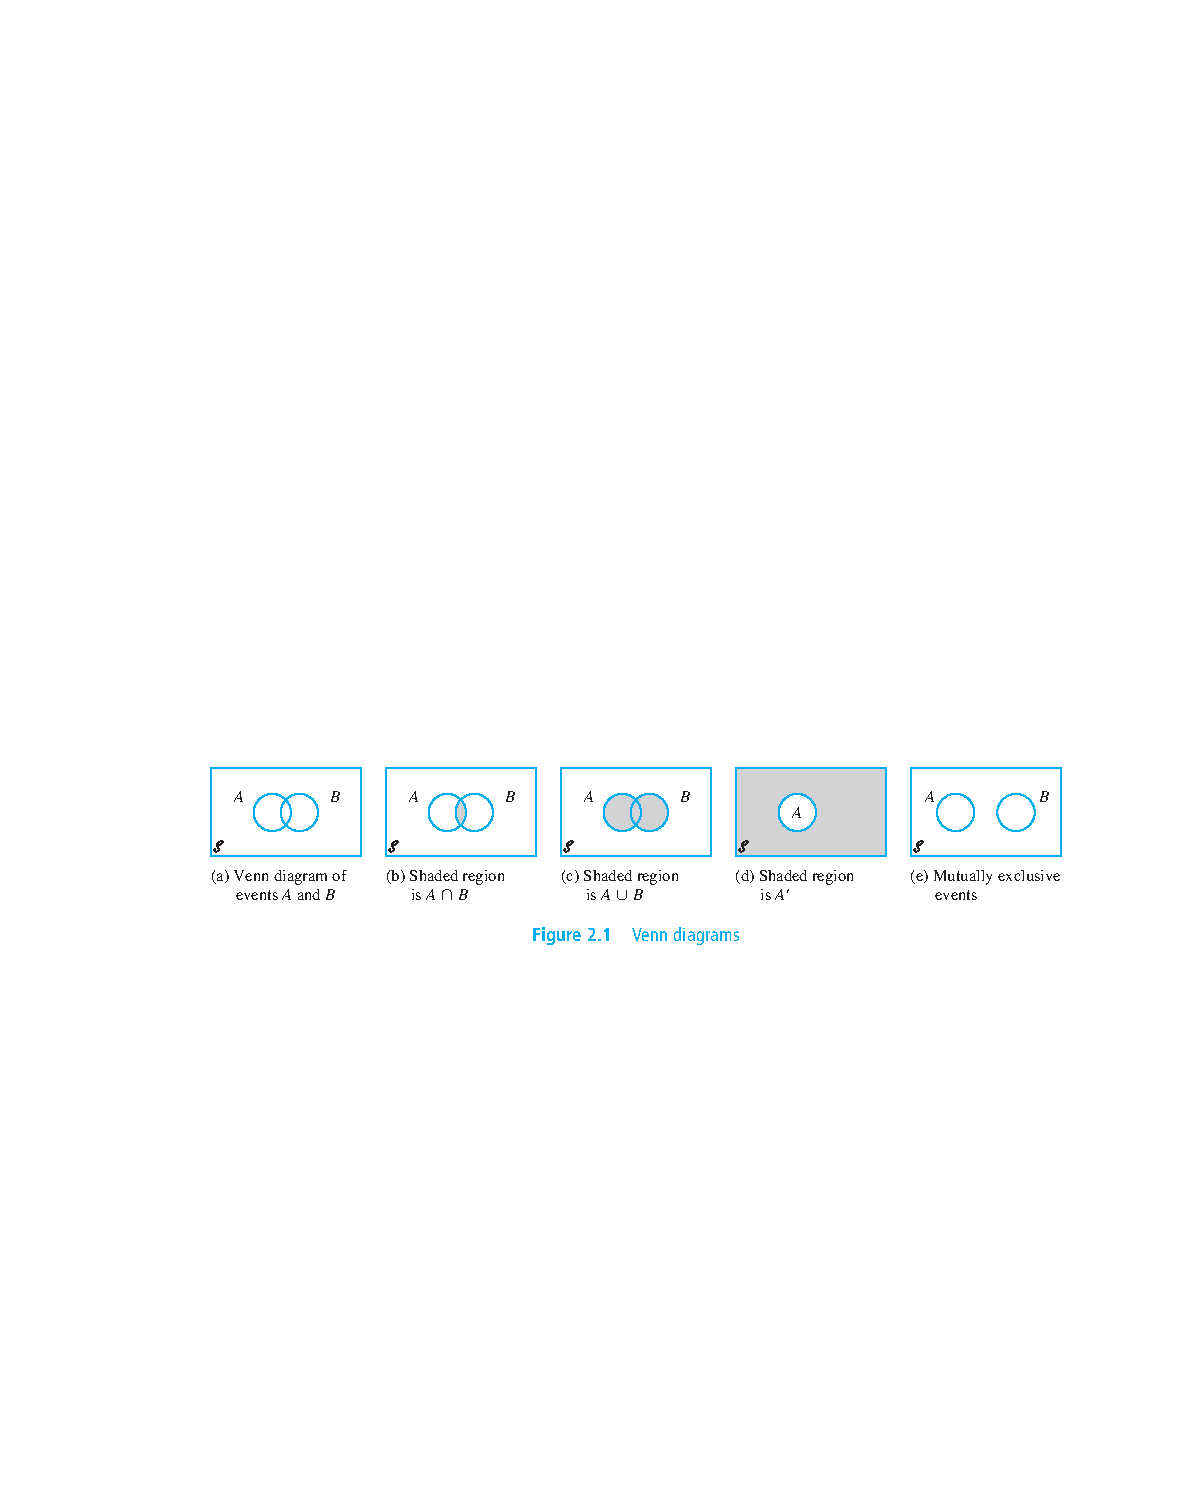
\includegraphics[width=15cm]{figures/venn_diagram.pdf}
\caption{Venn diagrams}
\label{fig:4}
\end{figure}

\begin{exmp}
  $(A\cup B)\cap C=(A \cap C)\cup(B \cap C)$
\end{exmp}


\section{Axioms, interpretations, and Properties of Probability}
Probability: Given a sample space $\mathcal{S}$, for any event $A\in \mathcal{S}$, assign a number, say $P(A)$, to it.
\begin{axio}
  For every event $A$, $P(A)\geq 0$.
\end{axio}

\begin{axio}
  $P(\mathcal{S})=1$
\end{axio}

\begin{axio}
If $A_1, A_2,A_3,\dots$is an infinite collection of disjoint events, then 
\[  P(A_1 \cup A_2\cup A_3 \cup \dots)=\sum_{i=1}^{\infty}P(A_i)	\]
\end{axio}

\begin{prop}
$P(\varnothing)=0$
\begin{proof}
Let $E_1=\varnothing,E_2=\varnothing,\dots E_n=\varnothing$
\[P(\varnothing \cup \varnothing \cup \dots \varnothing)=\sum_{i=1}^n P(\varnothing)\]
\[P(\varnothing)=nP(\varnothing)\]
\[P(\varnothing)=0\]
\end{proof}
\end{prop}

\begin{prop}
If $A$ and $B$ are disjoint, $P(A \cup B)=P(A)+P(B)$.
\begin{proof}
Let $E_1=A,E_2=B,E_3=\varnothing \dots E_n=\varnothing$. Then, we can prove it by Axiom 3.
\end{proof}
\end{prop}

\begin{exmp}
Flip a coin, $\mathcal{S}=\{H,T\}$
\[P(H)=0.89 \qquad P(T)=0.1\]
\[P(\mathcal{S})=P(H \cup T)=P(H)+P(T)=\boxed{0.99} \neq 1		\]

not a probability.
\end{exmp}

\begin{exmp}
Batteries come off an assembly line are tested one by one. The test will stop until a battery fails.
\[F:\text{faliure} \qquad S=\text{success}\]

Suppose $P(S)=0.99 \qquad P(F)=0.01$
\[\mathcal{S}=\{ F,SF,SSF,SSSF,\dots		\}\]
\[E_1=\{F\},E_2=\{SF\},E_3=\{SSF\},\dots		\]
\[P(\mathcal{S})=P(E_1 \cup E_2 \cup E_3 \dots)=P(E_1)+P(E_2)+P(E_3)+\dots\]
\[P(E_1)=0.01 \qquad P(E_2)=0.01\times0.99 \qquad P(E_3)=0.01\times 0.99^2\]
\[P(\mathcal{S})=0.01+0.99\times0.01+\dots=0.01\times\frac{1}{1-0.99}=1\]
\end{exmp}

\subsection{Interpreting Probability}
\begin{exmp}
If I flip a coin $10$ times, ref freq of H = \# of H /$10$. If I flip a coin $n$ times, ref freq of H = \# of H /$n$.

The probability of flipping a coin resulted in H= relative freq of H when $n\to \infty$. 
\[P(H)=\lim _{x \to \infty} \frac{\# of H}{n}\]
\end{exmp}

\subsection{How to calculate Properties of Probability}

\begin{prop}
$P(A')=1 -P(A) $
\begin{proof}
\[1=P(\mathcal{S})=P(A \cup A')=P(A)+P(A')\]
\end{proof}
\end{prop}
  
\begin{exmp}
Components connected in a series, each component has 0.3 probability of fail, and they fail independently.
   
\[A=\{\text{the system fails}\}\]
\[P(A)=P(\{ FSSSS,SFSSS,\dots\})\]
\[P(A)=1-P(\{\text{the system works}\})=1-P(SSSSS)=1-0.7^5\]
\end{exmp}
  
\begin{prop}
  If $A\cap B =\varnothing, P(A \cap B)=0 $
\end{prop}
  
\begin{prop}
 $ P(A \cup B)= P(A) +P(B) -P(A \cap B) $
\begin{proof}
Let $E = B \cap A' $, A and E are disjoint
  \[A \cup B = A \cup E\]
  \[P(A\cup B)=P(A \cup E)=P(A)+P(E)  \qquad (*)\]

Let $F= B\cap A$
  \[E \cup F =B \qquad E \cap F =\varnothing\]
  \[ P(B) = P(E \cup F)=P(E) + P(F)=P(E)+P(A\cap B)  \]
  \[P(E)= P(B)- P(A \cap B) \]

Plug in (*),\[  P(A \cup B)= P(A) +P(B) -P(A \cap B)  \]
\end{proof}
\end{prop}


\begin{exmp}
A card is drawn form a well-shuttled deck, what is the probability that it is a queen or a heart?
\begin{align*}
&Q=\{\text{the card is a Queen}\}\\
&H=\{\text{the card is a heart}\}
\end{align*}
\[P(Q \cup H)=P(Q)+P(H)-P(Q \cap H)=\frac{16}{52}\]
\end{exmp}

\begin{exmp}
In pccw, 80\% of the customers subscribed to cable TV. 30\% of the customers subscribed to Internet. 25\% of the customers subscribed to both.
Randomly select one customer, what is the chance that the person has either TV or Internet.
\[C=\{\text{the customers subscribed to cable TV}\}\]
\[I=\{\text{the customers subscribed to Internet} \}\]
\[P(C)=0.8 \qquad P(I)=0.3 \qquad P(C\cap I)=0.25\]
\[P(C\cup I)=P(C)+P(I)-P(C\cap I)=\boxed{0.85}\]
\end{exmp}

\begin{prop}
\[ P(A \cup B \cup C)=P(A)+P(B)+P(C)-P(A \cap B)-P(B \cap C)-P(C \cap A)+P(A \cap B \cap C) \]
\end{prop}

\begin{exmp}
C: Cable \qquad I: Internet \qquad T:Telephone.\footnote{Acutually a mistake $P(I\cap T)=0.4$}
\begin{align*}
&P(C)=0.8 \qquad P(I)=0.3 \qquad P(T)=0.5	\\
&P(C\cap I)=0.25 \qquad P(I\cap T)=0.4 \qquad P(C\cap T)=0.3\\
&P(C\cap I \cap T)=0.2
\end{align*}
\[P(C\cup I \cup T)=P(C)+P(I)+P(T)-P(C \cap I)-P(C \cap T)-P(I \cap T)+P(C \cap I \cap T)=\boxed{0.85}\]
\end{exmp}

\subsection{Determining Probabilities Systematically}
Any event $A$ is a union of simple events, i.e. with only one outcome. Then
\[P(A)=\sum_{E_i \in A}P(E_i),\]
and we just need to determine $P(E_i)$.

\begin{exmp}
Toss a dice, $\mathcal{S}=\{1,2,3,4,5,6\}$
\[P(\text{the spots}<4)\]
\[A=\{\text{the spot}< 4 \}=\{1,2,3\}\]
\[E_i=\{i\};\qquad i=1,2,3,4,5,6\]
\[A=E_1 \cup E_2 \cup E_3 \qquad  P(A)=P(E_1)+P(E_2)+P(E_3)\]

Suppose 
\[P(1)=P(2)=P(6)=\frac{1}{9}\]
\[P(3)=P(4)=P(5)=\frac{2}{9}\]
\[P(A)=P(1)+P(2)+P(3)=\frac{4}{9}\]
\end{exmp}

\subsection{Equally Likely Outcomes}
Suppose $\mathcal{S}$ has $N$ outcomes, $E_1,\dots E_N$, they are equally likely to occur, then
\[P(E_i)=\frac{1}{N} \qquad i=1,2,\dots\]

Then 
\[P(A)=\frac{\text{\# of outcome in A}}{N}\]

\begin{exmp}
Toss a pair of fair dices. What is the chance that the sum of spots is 3?
\[N=36 \qquad \mathcal{S}=\{(1,1),(1,2),\dots ,(6,6)\}\]
\[A=\{\text{the sum of spots is 3}\}=\{(1,2),(2,1)\}\]
\[P(A)=\frac{2}{36}\]
\end{exmp}

\begin{exmp}
What is the chance that the sum of spots $\leq 4$?
\[B=\{\text{the sum of spots}\leq 4\}=\{(1,1),(1,2),(1,3),(2,1),(2,2),(3,1)\}\]
\[P(B)=\frac{6}{36}\]
\end{exmp}

\section{Counting Techniques}
\begin{exmp}
A new guy comes to HK. If there are 3 brands of cell phone, 4 telephone companies offer mobile service.

\end{exmp}

\subsection{Product Rule}
Select two elements in a row. The first element has $n_1$ choices, the second has $n_2$ choices. Then the number of pairs $ = n_1 \cdot n_2$.

In general: suppose a set consists of $K$ ordered elements (K-tuples), 1st element has $n_1$ choices, 2nd element has $n_2$ choices, 3rd element has $n_3$ choices,\dots. Then the number of different K-tuples is $n_1 n_2 \dots n_k$.


\subsection{Permutations and Combinations}
\begin{exmp}
70 students in the room choose 4 students to form a committee (secretary, treasury, officer 1, officer 2).
\begin{enumerate}
\item How many possible committees with position assigned?
\[70 \times 69 \times 68 \times 67=\frac{70!}{66!} \]
\item How many possible committees without position assigned?
%\[{70 \choose 4} =\frac{70!}{4! \times 66!}\]
\[\binom{70}{4}=\frac{70!}{4! \times 66!}\]
\end{enumerate}
\end{exmp}

\begin{defn}
The number of \textbf{permutation} of size $k$ of $n$ objects is denoted as $P_{k,n}=\frac{n!}{(n-k)!}$.

In specific, $P_{n,n}=n!\qquad (0!=1)$
\end{defn}

\begin{defn}
Given $n$ distinct objects,any disordered subject of size $k$ is called a \textbf{combination} of size $k$. The number of combination of size $k$ of $n$ objects, is denoted as $C_{k,n}$ or $\binom nk=\frac{n!}{k!(n-k)!}$.
\end{defn}


\begin{exmp}
\[\{A,B,C,D,E\}\]
\begin{enumerate}
\item  Choose 3 letters, how many choices?
\[\binom 53 =10\]
\item  Choose 3 letters to form a word, how many different words?
\[P_{3,5}=60\]
\end{enumerate}
\end{exmp}

\begin{prop}
\[k!\times C_{k,n}=\binom nk \times k!=P_{k,n}\]
\end{prop}

\begin{exmp}[``Birthday Paradox"] 
365 different dates, $n$ students.
\begin{align*}
&P\{\text{at least two students share the same birthday}\}\\
&=1-P\{\text{every one has a diffrent birthday}\}\\
&=1-\frac{P_{n,365}}{365^n}
\end{align*}

If $n=50$, $P=97\%$

If $n=100$, $P=99.99997\%$
\end{exmp}


\section{Conditional Probability}
\begin{exmp}
52 cards. One card is dealt, and the another card is dealt.
\begin{enumerate}
\item P(the second card is 7 of clubs)
$=\frac{1}{52}$
\item P(the second card is 7 of clubs given the first is J of spade)
$=\frac{1}{51}$
\item P(the first card is J of spade, and the second card is 7 of clubs)
$=\frac{1}{P_{2,52}}=\frac{1}{52\times 51}$
\item P(the first card is J of spade)
$=\frac{1}{52}$
\end{enumerate}

So P(B given A)=$\frac{P(A \cap B)}{P(A)}$
\end{exmp}

\begin{exmp}
Fishing in the sea
\begin{center}
\begin{tabular}{c|c|c}
\hline
 & Walleye & Pike\\
 \hline
 Sam & 2 &3\\
 \hline
 I & 1 &5\\
 \hline
\end{tabular}
\end{center}

Randomly pick one, found, it is s Walleye. What is the chance that it is caught by me?
\begin{align*}
&A=\{\text{Walleye}\}\\
&B=\{\text{Caught by me}\}\\
&P(A)=\frac{3}{11} \qquad P(B)=\frac{6}{11}\\
&P(B\text{ given }A)=\frac{P(A \cap B)}{P(A)}=\boxed{\frac{1}{3}}
\end{align*}
\end{exmp}

\subsection{The Definition of Conditional Probability}
\begin{defn}
For any two events $A$ and $B$, with $P(B)>0$, the conditional probability of $A$ given that $B$ has occurred is defined by
\[P(A|B)=\frac{P(A \cap B)}{P(B)}\]
\end{defn} 

\begin{exmp}
Of all costumers purchasing computers, 60\% of them include M\$ Word; 50\% of them include M\$ Excel; 30\% of them include both.
\begin{align*}
&A=\{\text{Word is included}\} 	\\
&B=\{\text{Excel is included}\}	
\end{align*}
\[P(A|B)=0.6 \qquad P(B|A)=0.5\] 
\[P(A|B)\neq P(B|A)\]
\end{exmp}

\textbf{Recall}:
Axioms of probability

\begin{enumerate}
\item  For every event $A$, $P(A)\geq 0$.
\item  $P(\mathcal{S})=1$
\item
If $A_1, A_2,A_3,\dots$is an infinite collection of disjoint events, then 
\[  P(A_1 \cup A_2\cup A_3 \cup \dots\cup A_n)=\sum_{i=1}^{n}P(A_i)	\]
\end{enumerate}

Similarly,
\begin{enumerate}
\item  For every event $A$, $P(A|B)\geq 0$.
\item  $P(B|B)=1$
\item  If $A_1, A_2,A_3,\dots$is an infinite collection of disjoint events, then 
\[  P(A_1 \cup A_2\cup A_3 \cup \dots\cup A_n|B)=\sum_{i=1}^{n}P(A_i|B) \]
\end{enumerate}

\begin{exmp}
A new magazine publishes 3 columns: ``Art"(A), ``Boobs"(B), ``Cinema"(C). Research shows the reading habits:
\begin{center}
\begin{tabular}{ccccccc}
\hline
$A$ & $B$ & $C$ & $A\cap B$ & $A\cap C$ & $B\cap C$ & $A \cap B\cap C$\\
\hline
0.14&0.23&0.37&0.08&0.09&0.13&0.05\\
\hline
\end{tabular}.
\end{center}

Randomly select one reader

(1)
\[P(A|B)=\frac{P(A \cap B)}{P(B)}=\boxed{\frac{8}{23}}\]

(2)
\begin{align*}
P(A|B\cup C)&=\frac{P(A\cap (B\cup C) )}{P(B\cup C)}\\
&=\frac{P\big( (A\cap B)\cup(A \cap C) \big)}{P(B)+P(C)-P(B \cap C)}\\
&=\frac{P(A\cap B)+P(A\cap C)-P(A\cap B\cap C)}{P(B)+P(C)-P(B \cap C)}
\end{align*}

(3) $P(A|A \cup B \cup C)$: What is the probability that the reader read ``Art" Column given that  he/she reads at least one column?
\begin{align*}
P(A|A \cup B \cup C)&=\frac{P(A \cap (A \cup B \cup C) )}{P(A \cup B \cup C)}=\frac{P(A)}{P(A \cup B \cup C)}\\
&=\frac{P(A)}{P(A)+P(B)+P(C)-P(A \cap B)-P(B \cap C)-P(C \cap A)+P(A \cap B \cap C)}\\
&=\boxed{\frac{14}{49}}
\end{align*}

(4)
\begin{align*}
P(A \cup B |C)=&\frac{P((A \cup B)\cap C)}{P(C)}\\
=&\frac{P(A \cap C) +P(B \cap C)-P(A \cap B \cap C)}{P(C)}=\boxed{\frac{17}{37}}
\end{align*}
\end{exmp}

\subsection{The Multiplication Rule for $P(A\cap B)$}
\begin{prop}
\[P(A \cap B)=P(A)P(B|A)=P(B)P(A|B)\]
\end{prop}

\begin{exmp}
Two cards are dealt.

\[P(\text{1st is J of spade and 2nd is 7 of heart})=P(A)P(B|A)=\frac{1}{52} \times \frac{1}{51}\]
\end{exmp}

\begin{exmp}
Same scenario

\[ A=\{\text{1st is a club}\} \]
\[ B=\{\text{2nd is a club}\}\]
\[P(A\cap B)=P(A)P(B|A)=\frac{13}{52} \times \frac{12}{51}\]
\[C=\{\text{3rd card is a heart}\} \]
\[P(A \cap B\cap C)=P(A\cap B)P(C|A \cap B)=P(A)P(B|A)P(C|A \cap B)=\frac{13}{52} \times \frac{12}{51} \times \frac{13}{50}\]
\end{exmp}

\begin{prop}
\[P(A_1 \cap A_2 \dots \cap A_k)=P(A_1)P(A_2|A_1)P(A_3|A_1\cap A_2)\dots P(A_k|A_1\cap A_2\dots\cap A_{k-1})\]
\end{prop}

\begin{exmp}
Same scenario
\begin{align*}
& A=\{\text{1st is a club}\} \\
& B=\{\text{2nd is A of club}\} \\
& C=\{\text{3rd is 2 of club}\} \\
\end{align*}
\[ P(A \cap B\cap C)=P(C)P(B|C)P(A|B\cap C)=\frac{1}{52}\times\frac{1}{51}\times\frac{11}{50} \]

Introduce $D=\{\text{1st is either 3,4,\dots K of club}\}$
\[P(A \cap B\cap C)=P(D\cap B\cap C)=\frac{11}{52}\times\frac{1}{51}\times\frac{1}{50}\]
\end{exmp}

\subsection{Bayes' Theorem}
\begin{theo}  [The Law of Total Probability]
  Let $A_1, . . . , A_k$ be mutually exclusive and exhaustive events. Then for any other event $B$,
  \[ P(B)=\sum_{i=1}^{k} P(B|A_i)P(A_i)\]
\end{theo}

\begin{exmp}
A store sells 3 brands of game consoles

\begin{center}
 \begin{tabular}{l|ccc}
 \hline
 Brand & 1 & 2 & 3 \\
 \hline
 Proportion & 50\% & 30\% & 20\%\\
 \hline
 \end{tabular}  
\end{center}

A one year warranty is offered, known 

\begin{center}
    \begin{tabular}{l|ccc}
    \hline
    Brand & 1 & 2 & 3 \\
    \hline
    Under warranty & 25\% & 20\% & 10\%\\
    \hline
  \end{tabular}
\end{center}
  \[A_i=\{\text{bought brand }i\} \qquad i=1,2,3\]
  \[B=\{\text{needs repaire under warranty}\} \]
  \[P(A_1)=0.5 \qquad P(A_2)=0.3 \qquad P(A_3)=0.2\]
  \[P(B|A_1)=0.25 \qquad P(B|A_2)=0.2 \qquad P(B|A_3)=0.1\]
  
  Q1:\[P(B'|A_1)=1-P(B|A_1)=0.75\]

  Q2:\[P(B)=P(A_1)P(B|A_1)+P(A_2)P(B|A_2)+P(A_3)P(B|A_3)=0.205\]

  Q3:\begin{align*}
  &P(A_1|B)=\frac{P(A_1 \cap B)}{P(B)}=\frac{P(A_1)P(B|A_1)}{P(B)}=0.61\\
  &P(A_2|B)=0.29 \\
  &P(A_3|B)=0.10\\
  \end{align*}
\end{exmp}

\begin{theo} [Bayes' Theorem]
  \[P(A_i|B)=\frac{P(A_i \cap B)}{P(B)}=\frac{P(A_i)P(B|A_i)}{\sum_{i=1}^k P(A_k)P(B|A_i)}    \]
\end{theo}

\begin{exmp}
$\frac{1}{1000}$ adults has a rare disease.

99\% of people with the disease can be found positive

20\% of people without the disease can be found positive

Randomly select a person and test him. Suppose the result is positive. What is the chance that he really has the disease? 

Let
\[	A=\{\text{the individual has the disease} \}		\]
\[	A'=\{\text{the individual does not have the disease} \}		\]
\[	B=\{\text{that positive} \}		\]
\[	P(A)=\frac{1}{1000} \qquad P(B|A)=0.99 \qquad P(B|A')=0.20	\]

Question:
\[	P(A|B)=\frac{P(A \cap B)}{P(B)}=\frac{P(A)P(B|A)}{P(A)P(B|A)+P(A')P(B|A')}		\]

Because $A$ and $A'$ are portions of $\mathcal{S}$
\[	=\frac{0.001\times 0.99}{0.001\times 0.99+ 0.999\times 0.2}=0.493\%		\]
\end{exmp}
\section{Independence}
\begin{defn}
Two events A and B. If A and B are \textbf{independent}, then
\[P(A\cap B)=P(A)P(B) \]

Note that $P(A \cap B)=P(A)P(B|A)$ apply for any condition.
\[  P(B)=P(B|A), \]
event $A$ has nothing to do with event B.
\end{defn}

\begin{exmp}
  Roll a dice once. $P(i)=\frac{1}{6}; i=1,2,\dots,6$
  \[  A=\{2,4,6\},   B=\{1,2,3\},   C=\{1,2,3,4\} \]
  \[  P(A)=\frac{3}{6}=\frac{1}{2} \]
  \[ P(A|B)=\frac{P(A\cap B)}{P(B)}=\frac{1/6}{3/6}=\frac{1}{3} \]
  \[ P(A|C)=\frac{P(A\cap C)}{P(C)}=\frac{2/6}{4/6}=\frac{1}{2} \]

So $A$ and $C$ are independent. $A \not\!\perp\!\!\!\perp B$
\end{exmp}

\begin{prop}
If $A$ and $B$ are independent,
\begin{itemize}
  \item $A'$ and $B'$ are independent,
  \item $A'$ and $B$ are independent,
  \item $A$ and $B'$ are independent.
\end{itemize}
\end{prop}

\begin{exmp}
  Toss a fair coin repeatedly until the first H occurs.
  \[A=\{\text{at least 5 tosses result in the first H}\}\]
  \[P(A)= \quad ?\]
\begin{solution}	 
Assume the tossing are independent.
\[A=\{TTTTH\}\cup	\{TTTTTH\} \cup \dots	\]
\begin{align*}
P(A)&=P(\{TTTTH\})+\dots =(P(T))^4 P(H)+(P(T))^5 P(H)\\
&=\left(\frac{1}{2}\right)^5+\left(\frac{1}{2}\right)^6+\dots=\frac{1}{16}
\end{align*}
\end{solution}
\end{exmp}

\subsection{Independence of More Than Two Events}
\begin{defn}
$A_1,A_2,\dots A_k$ are events. If for any indices $i,\dots, i_k$
\[P(A_1 \cap A_2 \cap \dots A_k)=P(A_1)P(A_2)\dots P(A_k)\]

Then $A_1,A_2,\dots A_k$ are said to be mutually independent.
\end{defn}

\begin{exmp}
Component works with probability 0.9, and they work independently.
\[P(\text{system works})\]
\begin{solution}	
Let
\begin{align*}
&A_i=\{ \text{the }i\text{th component works} \}	\\
&P(A_i)=0.9	\\
&P(\text{system works})=P\left( (A_1 \cap A_2)\cup(A_3 \cap A_4) \right)=0.9639\\
\end{align*}
\end{solution}
\end{exmp}

\section{Challenge Question 1}
Monty Hall problem. \url{https://en.wikipedia.org/wiki/Monty_Hall_problem}


\section{Problem in Previous Mid-term Test}
 \begin{exmp}
 \begin{align*}
   &D=\{\text{David makes a right decision}\}	\\
   &J=\{\text{John makes a right decision}\}	\\
   &P=\{\text{Peter makes a right decision}\}	
 \end{align*}

David and Peter make decision independently.
  \[  P(D) = 0.7 \qquad P(D|J)=0.9 \qquad P(D'|J')=0.8  \]
  \[  P(J|P)=0.3 \qquad P(J'|P')=0.2 \qquad P(D \cap J\cap P)=0.1 \]

  Question: Find
  (1) $P(J)$; 
  (2) $P(P)$; 
  (3) $P(\text{at least two make right decision})$.
\end{exmp}

\begin{solution}
  (1)
  \begin{align*}
  &0.9=P(D|J)=\frac{P(D \cap J)}{P(J)}  \\
  &0.8=P(D'|J')=\frac{P(D'\cap J')}{P(J')}=\frac{P(D\cup J)'}{1-P(J)}=\frac{1-P(D\cup J)}{1-P(J)}
  \end{align*}
  \[P(D\cup J)=P(D)+P(J)-P(D \cap J)=0.7+P(J)-P(D \cap J)\]
  \[P(J)=\frac{5}{7}\]

  (2) Similar to (1)

  (3)
  \[P(\text{at least two make right decision})\]
  
Method A:
\begin{align*}
  &=1-P(\text{no more than 1 make right decisions})\\
  &=1-P(D \cap J \cap P')-P(D' \cap J \cap P')-P(D' \cap J' \cap P)-P(D' \cap J' \cap P')
\end{align*}

Method B:
\[ =P(A \cap B)+P(B \cap C) + P(C \cap A)-2 P(A\cap B \cap C)\]
\end{solution}